%------------------------------------------------
\section{Hashing}
%------------------------------------------------

\subsection{Hash Function}

\begin{frame}


Fonction qui:
\begin{itemize}
    \item prends en entrée des données de taille arbitraire
    \item fait correspondre une sortie de taille fixe
    \item est déterministe
\end{itemize}

\begin{center}
\begin{minipage}[c]{0.7\linewidth}
% Style definition file generated by highlight 3.18, http://www.andre-simon.de/ 

% Highlighting theme: Kwrite Editor 

\newcommand{\hlstd}[1]{\textcolor[rgb]{0,0,0}{#1}}
\newcommand{\hlnum}[1]{\textcolor[rgb]{0.69,0.49,0}{#1}}
\newcommand{\hlesc}[1]{\textcolor[rgb]{1,0,1}{#1}}
\newcommand{\hlstr}[1]{\textcolor[rgb]{0.75,0.01,0.01}{#1}}
\newcommand{\hlpps}[1]{\textcolor[rgb]{0.51,0.51,0}{#1}}
\newcommand{\hlslc}[1]{\textcolor[rgb]{0.51,0.51,0.51}{\it{#1}}}
\newcommand{\hlcom}[1]{\textcolor[rgb]{0.51,0.51,0.51}{\it{#1}}}
\newcommand{\hlppc}[1]{\textcolor[rgb]{0,0.51,0}{#1}}
\newcommand{\hlopt}[1]{\textcolor[rgb]{0,0,0}{#1}}
\newcommand{\hlipl}[1]{\textcolor[rgb]{0,0.34,0.68}{#1}}
\newcommand{\hllin}[1]{\textcolor[rgb]{0.33,0.33,0.33}{#1}}
\newcommand{\hlkwa}[1]{\textcolor[rgb]{0,0,0}{\bf{#1}}}
\newcommand{\hlkwb}[1]{\textcolor[rgb]{0,0.34,0.68}{#1}}
\newcommand{\hlkwc}[1]{\textcolor[rgb]{0,0,0}{\bf{#1}}}
\newcommand{\hlkwd}[1]{\textcolor[rgb]{0,0,0.51}{#1}}
\definecolor{bgcolor}{rgb}{0.88,0.92,0.93}


\noindent
\ttfamily
\hlstd{}\hlslc{\#!\ /usr/bin/python\ {-}u}\hspace*{\fill}\\
\hlstd{}\hspace*{\fill}\\
\hlkwa{def\ }\hlstd{}\hlkwd{hash\textunderscore function}\hlstd{}\hlopt{(}\hlstd{text}\hlopt{):}\hspace*{\fill}\\
\hlstd{}\hlstd{\ \ \ \ }\hlstd{out\ }\hlopt{=\ }\hlstd{}\hlnum{0}\hspace*{\fill}\\
\hlstd{}\hlstd{\ \ \ \ }\hlstd{}\hlkwa{for\ }\hlstd{c\ }\hlkwa{in\ }\hlstd{text}\hlopt{:}\hspace*{\fill}\\
\hlstd{}\hlstd{\ \ \ \ \ \ \ \ }\hlstd{out\ }\hlopt{+=\ }\hlstd{}\hlkwb{ord}\hlstd{}\hlopt{(}\hlstd{c}\hlopt{)}\hspace*{\fill}\\
\hlstd{}\hlstd{\ \ \ \ }\hlstd{}\hlkwa{return\ }\hlstd{out\ \%\ }\hlnum{100}\hspace*{\fill}\\
\hlstd{}\hspace*{\fill}\\
\hlkwa{print\ }\hlstd{}\hlkwd{hash\textunderscore function}\hlstd{}\hlopt{(}\hlstd{}\hlstr{"hello"}\hlstd{}\hlopt{)}\hlstd{\ \ \ \ }\hlopt{}\hlstd{}\hlslc{\#\ {-}$>$\ 32}\hspace*{\fill}\\
\hlstd{}\hlkwa{print\ }\hlstd{}\hlkwd{hash\textunderscore function}\hlstd{}\hlopt{(}\hlstd{}\hlstr{"world"}\hlstd{}\hlopt{)}\hlstd{\ \ \ \ }\hlopt{}\hlstd{}\hlslc{\#\ {-}$>$\ 52}\hspace*{\fill}\\
\hlstd{}\hlkwa{print\ }\hlstd{}\hlkwd{hash\textunderscore function}\hlstd{}\hlopt{(}\hlstd{}\hlstr{"!"}\hlstd{}\hlopt{)}\hlstd{\ \ \ \ \ \ \ \ }\hlopt{}\hlstd{}\hlslc{\#\ {-}$>$\ 33}\hlstd{}\hspace*{\fill}\\
\mbox{}
\normalfont
\normalsize

\end{minipage}
\end{center}

\end{frame}

%------------------------------------------------




\subsection{Cryptographic Hash Function}
\begin{frame}
\frametitle{Introduction}
\begin{itemize}
    \item Une fonction de hachage avec les propriétés:
    \begin{itemize}
        \item Est rapide à calculer quelque soit la taille de l'entrée
        \item A un espace de sortie suffisamment large
        \item Un petit changement dans l'entrée provoque une cascade de changements en sortie
        \item En utilisant la sortie, il est difficile de re-créer l'entrée
        \item Si on a l'entrée et la sortie, il est difficile de trouver une autre entrée avec la même sortie
    \end{itemize}
\end{itemize}
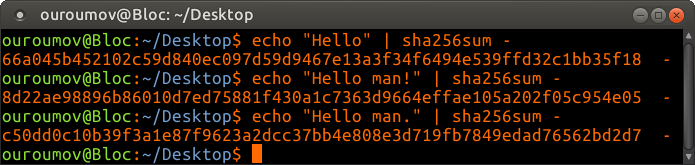
\includegraphics[scale=.5]{res/sha256sum}
\end{frame}


%------------------------------------------------


\subsection{Password Hash Function}
\begin{frame}
Une fonction de hachage pour mots de passe doit:
\begin{itemize}
    \item Avoir les propriétés d'une fonction de hachage cryptographique
    \item Utiliser un Sel concaténé avec le mot de passe
    \item Être configurable pour pouvoir consommer:
    \begin{itemize}
        \item Une quantité de mémoire arbitraire
        \item Un nombre de cycles CPU arbitraire
    \end{itemize}
\end{itemize}

\begin{center}
BCrypt Hash Function, cost level 10
\end{center}
\resizebox{\textwidth}{!}{%
    \begin{tabular}{ c | c | c }
    Password & Salt & Hash \\ \hline
    \texttt{Passw0rd} & \textcolor{blue}{\texttt{Q/AzxLshsyaAqptlgni74u}} & \texttt{\$2a\$10\$}\textcolor{blue}{\texttt{Q/AzxLshsyaAqptlgni74u}}\textcolor{green}{\texttt{N5WQrGCW176CPbPSVqrt/pUNS7HW9tu}} \\ \hline
    \texttt{lolwhat}  & \textcolor{blue}{\texttt{7JYaQZA9w/PGfv4C0ab92O}} & \texttt{\$2a\$10\$}\textcolor{blue}{\texttt{7JYaQZA9w/PGfv4C0ab92O}}\textcolor{green}{\texttt{qmH.YFrQmucp1wqRfUEd3KHI/ty6dHm}} \\ \hline
    \texttt{lolwhat}  & \textcolor{blue}{\texttt{02h4313J6Qgs/3daZ/iaze}} & \texttt{\$2a\$10\$}\textcolor{blue}{\texttt{02h4313J6Qgs/3daZ/iaze}}\textcolor{green}{\texttt{9RJR3EIblB6HZRX8zAWuP3TNKSY1zDu}} \\ \hline
    \end{tabular}
}

\end{frame}

%------------------------------------------------
